\subsection{M.PC.CO - Correttezza ortografica}

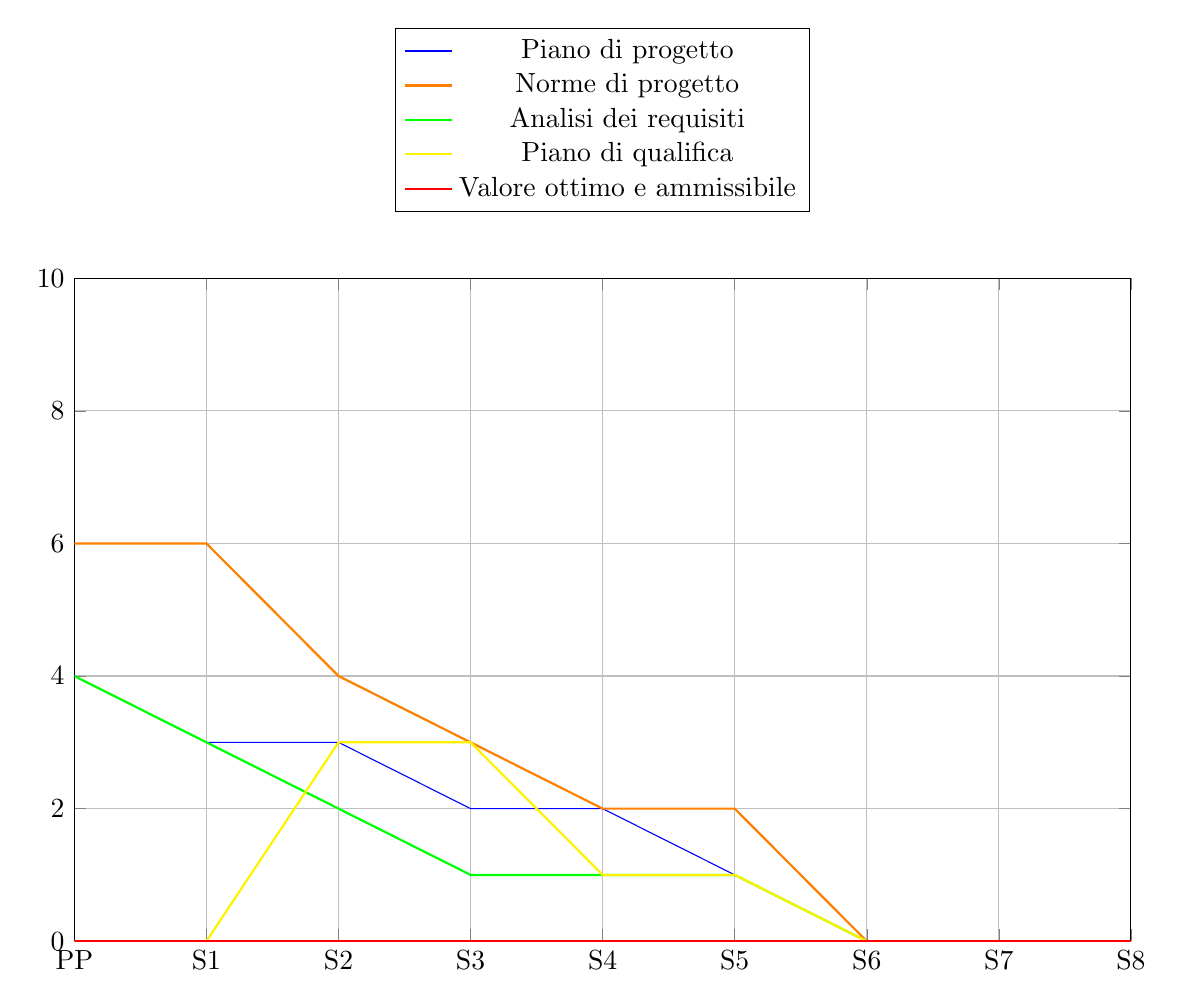
\begin{tikzpicture}
    \begin{axis}[
        width=15cm, height=10cm,
        ymin=0, ymax=10,
        xmin=0, xmax=8,
        xtick={0, 1, 2, 3, 4, 5, 6, 7, 8},
        xticklabels={ PP, S1, S2, S3, S4, S5, S6, S7, S8},
        xlabel={},
        ylabel={},
        grid=major,
        scaled ticks=false,
        legend style={at={(0.5,1.1)}, anchor=south, legend columns=1},
    ]
    \addplot[color=blue] coordinates {(0, 4) (1, 3) (2, 3) (3, 2) (4, 2) (5, 1) (6, 0) (7, 0) (8, 0)};
    \addlegendentry{Piano di progetto}
    \addplot[orange, thick] coordinates {(0, 6) (1, 6) (2, 4) (3, 3) (4, 2) (5, 2) (6, 0) (7, 0) (8, 0)};
    \addlegendentry{Norme di progetto}
    \addplot[green, thick] coordinates {(0, 4) (1, 3) (2, 2) (3, 1) (4, 1) (5, 1) (6, 0) (7, 0) (8, 0)};
    \addlegendentry{Analisi dei requisiti}
    \addplot[yellow, thick] coordinates {(0, 0) (1, 0) (2, 3) (3, 3) (4, 1) (5, 1) (6, 0) (7, 0) (8, 0)};
    \addlegendentry{Piano di qualifica}
    \addplot[red, thick] coordinates {(0, 0) (1, 0) (2, 0) (3, 0) (4, 0) (5, 0) (6, 0) (7, 0) (8, 0)};
    \addlegendentry{Valore ottimo e ammissibile}
    \end{axis}
\end{tikzpicture}
\subsubsection{RTB}
Si può notare che la quantità di errori grammaticali presenti nei documenti era inizialmente elevata. 
Tuttavia, sono stati effettuati controlli manuali durante lo \glossario{Sprint} 2 e lo \glossario{Sprint} 4 per ridurre il numero di errori. 
Inoltre, durante lo \glossario{Sprint} 5 è stata completata l'implementazione della \glossario{GitHub Action} per il controllo grammaticale automatico, garantendo così un monitoraggio continuo e più efficace della qualità linguistica dei documenti.